\documentclass[conference]{IEEEtran}

\usepackage[numbers]{natbib}
\usepackage{amsmath,amssymb,amsfonts}
\usepackage{algorithmic}
\usepackage{graphicx}
\usepackage{textcomp}
\usepackage{xcolor}
\usepackage{hyperref}
\usepackage{tikz}
\usepackage{multirow}
\usepackage{pgfplots}
\pgfplotsset{compat=1.18}
\usepackage[acronym]{glossaries}

\hypersetup{
    colorlinks=true,
    allcolors=.,
    urlcolor=blue}

\begin{document}

\newcommand{\authcite}[1]{\citeauthor{#1} \cite{#1}}

\title{A systematic review on produce defect detection and quality assessment using artificial intelligence}

\author{
    \IEEEauthorblockN{1\textsuperscript{st} João Silva}
    \IEEEauthorblockA{\textit{Departamento de Engenharia Informática} \\
    \textit{Instituto de Superior de Engenharia do Porto}\\
    1150425@isep.ipp.pt}
    \\
    \IEEEauthorblockN{3\textsuperscript{th} Nuno Costa}
    \IEEEauthorblockA{\textit{Departamento de Engenharia Informática} \\
    \textit{Instituto de Superior de Engenharia do Porto}\\
    1171584@isep.ipp.pt}
    \\
    \IEEEauthorblockN{5\textsuperscript{th} Diogo Formosinho}
    \IEEEauthorblockA{\textit{Departamento de Engenharia Informática} \\
    \textit{Instituto de Superior de Engenharia do Porto}\\
    1210056@isep.ipp.pt}
    \and
    \IEEEauthorblockN{2\textsuperscript{nd} João Santos}
    \IEEEauthorblockA{\textit{Departamento de Engenharia Informática} \\
    \textit{Instituto de Superior de Engenharia do Porto}\\
    1161023@isep.ipp.pt}
    \\
    \IEEEauthorblockN{4\textsuperscript{th} José Araújo}
    \IEEEauthorblockA{\textit{Departamento de Engenharia Informática} \\
    \textit{Instituto de Superior de Engenharia do Porto}\\
    1180943@isep.ipp.pt}
    \\
    \IEEEauthorblockN{6\textsuperscript{th} Francisco Cabrita}
    \IEEEauthorblockA{\textit{Departamento de Engenharia Informática} \\
    \textit{Instituto de Superior de Engenharia do Porto}\\
    1210058@isep.ipp.pt}
}
\maketitle

\begin{abstract}

\end{abstract}

\begin{IEEEkeywords}
\end{IEEEkeywords}

\section{Introduction}

Agriculture is one of the most important economic activities, sustaining livelihoods by securing food production and providing income \cite{FDES-1}, with a global gross value of 4.145 trillion US dollars in 2020 \cite{FAO1}. This sector has and continues to undergo a process of steady industrialization, through the increase of commercial farm size, commodity specialization and increase capital availability, among other factors \cite{10.2307/1243439}. This industrialization has caused an explosive increase in productivity for nearly all agricultural activity \cite{owidagriculturalproduction}. In order to take full advantage of this increased productivity, improvements are also required in the infrastructure and post harvest processes of a given agricultural unit, before the produce reaches the final consumer \cite{Food_and_Agriculture_Organization_of_the_United_Nations2010-hb}. With this, the post-harvest process has become crucial to reduce waste, preserve said foods and provide the end consumer with fresh, quality items \cite{foods6010008}. The previously mentioned improvements have materialized into facilities in which the produce can be stored, cleaned, prepared, sorted and packaged. However, with the large throughput of produce being processed in the aforementioned facilities, there is a need for systems that effectively monitor and sort said produce, taking into account defects and overall quality \cite{Mahalik2009}.

Furthermore, markets are usually regulated to include minimum requirements on produce quality and appearance, such as European Commission Implementing Regulation (EU) 543/2011, which sets out minimum quality requirements for a variety of produce, such as intactness, soundness and cleanliness \cite{eu-5432011}. In order to abide by the aforementioned regulation, producers must consider travel time and the possibility of spoilage within that time frame \cite{biv081}. Small defects in produce expand over time and can potentially spoil the whole item (be it a single produce item or a packaged set of items). Detection systems are already in place in post harvesting processes in the horticultural sector, identifying pathological, mechanical, physiological and internal defects \cite{Nturambirwe2020}.

The purpose of this work is to understand what factors can be monitored to ascertain the quality or defect presence in produce, what techniques and technologies are available to analyse and monitor produce in a industrial environment and how is artificial intelligence and related fields enhancing the usage of said technologies. To do this, three research questions are presented, and existing studies that may answer these questions are analysed and discussed in order to reach an overview of the current state of the art in the topics of produce quality analysis and defect detection using artificial intelligence, the evolution of the domain and their application in the post-harvest processing field.

The remainder of this document is structured in 4 sections:
\begin{itemize}
	\item Section \ref{sec:meth}, in which the procedure taken in this systematic review is presented in detail and all steps of the process are accounted for. In this section, we go from the definition of the research questions to the selection of the works to be included in this review, while explicating the inclusion and exclusion criteria and the data sources considered.
	\item Section \ref{sec:res}, in which we show which answers to the different research questions are proposed by the analysed studies to the best of our knowledge.
	\item Section \ref{sec:disc}, in which we take a deeper look at these studies and identify potential challenges and future directions for research.
	\item Section \ref{sec:conc}, which outlines the Conclusions and Future Work.
\end{itemize}

\section{Method}
\label{sec:meth}

The literature review will focus on the analysis of existing detection systems for the aforementioned situations, in order to assess how they answer to the research questions and how, if any, artificial intelligence is implemented in these systems. Analysing the challenges these systems face will allow us to establish how, and if, artificial intelligence can improve on existing systems and overcome the challenges set forth previously. Furthermore, the application context of this work lies in the field of artificial intelligence in detection systems in food processing operations and therefore existing works in this area will also be explored.
The goal of a systematic review of the literature is to extract, analyse and interpret a corpus of work pertaining to a specific field of study. Systematic reviews are meant to be through and to follow a sequential, detailed, specific and repeatable workflow that allows other researchers to achieve similar results. The methodology described by Kitchenham \cite{kitch} proposes that systematic reviews should follow a number of steps:
\begin{itemize}
	\item Development of the review protocol (including rationale and research questions);
	\item Processing;
	\item Analysis;
	\item Demonstration of the research's results;
\end{itemize}
With this such, this review starts by presenting the Research Questions and the motivating problem. Then, the data sources selected for this review will be presented, along with the process of selecting and using the most adequate combination of search terms that generated a query that could be equally used in the different data sources. Inclusion and Exclusion criteria, along with quality assessment criteria are described. Finally, a detailed account of the data extraction process is given, showing how the articles found in those data sources were continuously filtered until the final number of articles to review is reached.

\subsection{Research Questions}

For the purpose of this systematic review, we define the main research question as: ``What are the current applications of artificial intelligence based detection systems in the post harvest quality assurance processes?''. In order to properly answer this question, we can divide the main question into three more focused questions, which can be found in Table~\ref{tab:resquest}. The first question is mainly concerned with the physical factors that affect the quality analysis and defect detection processes. The second question then concerns itself with researching existing systems that utilize the aforementioned factors to detect defects and analyse the quality of produce. Finally, the last question focuses on identifying on which of these available systems integrate artificial intelligence, and to what degree this integrations provides usefulness to the overall system.

\begin{table*}
    \caption{Research Questions}
    \label{tab:resquest}

    \begin{tabular}{ll}
    \hline
        & \textbf{Research Question}\\
    \hline
        RQ1 & What objectives can be defined in the context of quality assessment or defect presence in produce? \\
        RQ2 &  What techniques and technologies are available to analyse and monitor produce in a industrial environment?\\
        RQ3 & What techniques and technologies previously researched utilize artificial intelligence, and how? \\
    \hline
    \end{tabular}
\end{table*}

\subsection{Data Sources}

The first step in the systemic review process is to identify the used data sources. It is advisable
to maintain a small number of comprehensible data sources, in order to maintain clarity and rigour \cite{Par2015}. Table~\ref{tab:edata} identifies the electronic databases chosen for this study. Within these data sources exist a degree of overlap, which will be accounted for in a following step.

\begin{table*}
    \caption{Electronic databases}
    \label{tab:edata}

    \begin{tabular}{lll}
    \hline
        Identifier & Database & URL \\
    \hline
        DS1 & ACM Digital Library & \url{https://dl.acm.org/} \\
        DS2 & IEEE Explore & \url{https://ieeexplore.ieee.org/} \\
    \hline

    \hline
    \end{tabular}
\end{table*}

\subsection{Search Terms}

Considering the application field of this research, along with the aforementioned questions, a number of domains were selected to assess not only how many studies have been performed, but how their combination affects the number of results. With this, consider the following domain selection and keywords, per Table~\ref{tab:resdom}.

\begin{table*}
	\caption{Domains and keywords used to select search terms}
	\label{tab:resdom}

	\begin{tabular}{ll}
	\hline
		Domain & Keywords \\
	\hline
		Artificial Intelligence & (``Artificial Intelligence'' OR ``Machine Learning'') \\
		Produce & (``Fruits'' OR ``Vegetables'' OR ``Berries'') \\
		Quality, Defects & (``Quality'' OR ``Defect'') \\
		Detection, Sorting & (``Classification'' OR ``Detection'' OR ``Grading'' OR ``Sorting'') \\
	\hline
	\end{tabular}
\end{table*}

Search terms were applied to Title, Abstract and Keywords. Different combinations of these domains were attempted and evaluated until a final search query was reached. Refer to Table~\ref{tab:resres} for the results of these attempts.

\begin{table*}[]
\caption{Combination of domains and respective results}
\label{tab:resres}
\begin{tabular}{llll}
\hline
\multirow{2}{*}{Domains}            & \multicolumn{3}{l}{Results} \\ \cline{2-4} 
                                    & ACM     & IEEE    & Total   \\ \hline
Artificial Intelligence             & 122,298 & 420,518 & 542,816 \\
Produce                             & 492,658 & 7,183   & 499,841 \\
Quality, Defects                    & 231,926 & 466,142 & 698,068 \\
Detection, Sorting                  & 246,506 & 747,608 & 994,114 \\
Artificial Intelligence AND Produce & 892     & 926     & 1,818   \\
Produce AND Quality, Defects        & 1,847   & 1,271   & 3,118   \\
Produce AND Quality, Defects AND Detection, Sorting                             & 1004 & 557 & 1,561 \\
Artificial Intelligence AND Produce AND Quality, Defects AND Detection, Sorting & 379  & 189 & 568   \\ \hline
\end{tabular}
\end{table*}

As can be inferred from Table~\ref{tab:resres}, we see that each individual domain provides a large volume of results. As such, the intersection of all domains provides us with a sufficient number of results that are more focused than other intersections, with some but no all defined domains. The final used query is as follows:

\begin{quote}
 (``Artificial Intelligence'' OR ``Machine Learning'') AND (``Fruits'' OR ``Vegetables'' OR ``Berries'') AND (``Quality'' OR ``Defect'') AND (``Classification'' OR ``Detection'' OR ``Grading'' OR ``Sorting'')
\end{quote}

\subsection{Quality assessment: inclusion and exclusion criteria}

In order to assess if a specific article should be included in this review, a set of rules were devised. These will evaluate a number of parameters unrelated to the actual content of the article (e.g. peer-review status, release format, article quality and relevance). Table~\ref{tab:inccrit} and Table~\ref{tab:exccrit} showcase the inclusion and exclusion criteria used, respectively.

\begin{table*}
	\caption{Inclusion Criteria}
	\label{tab:inccrit}

	\begin{tabular}{ll}
	\hline
		 & Inclusion Criteria \\
	\hline
		IC1 & The source belongs to the field of agricultural/food engineering  \\
		IC2 & The source describes a novel contribution to the fields of study \\
		IC3 & The source describes a methodology or system for produce quality control or defect detection, including novel sensor and software components \\
		IC4 & The source describes what factors are being measured in order to obtain the results described \\
	\hline
	\end{tabular}
\end{table*}

\begin{table*}
	\caption{Exclusion Criteria}
	\label{tab:exccrit}

	\begin{tabular}{ll}
	\hline
		 & Exclusion Criteria \\
	\hline
		EC1 & The source is over 5 years old \\
		EC2 & The source is a systematic review \\
		EC3 & The source is not written in English \\
		EC4 & The contribution to the fields of agricultural/food engineering and artificial intelligence is not clear of not the focus of the source \\
		EC5 & The source does not provide sufficient information on the specifications of the techniques, methodologies or systems used or developed \\
	\hline
	\end{tabular}
\end{table*}

\subsection{Data Extraction}

Figure~\ref{fig:elig} represents the process used to undertake this systematic review.

\begin{figure*}[tb]
	\centering
	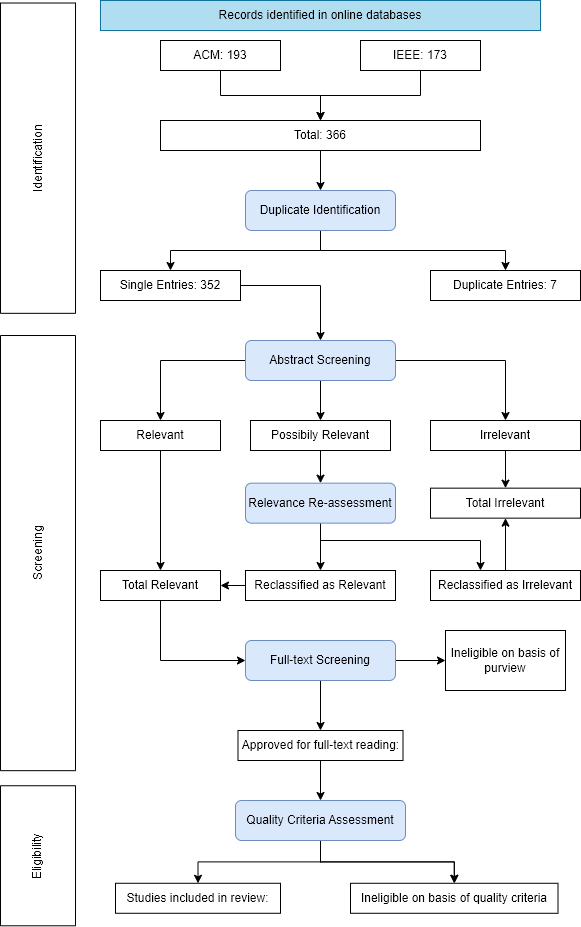
\includegraphics[width=0.45\textwidth]{images/eligibilityprocess.png}
	\caption{Eligibility Process Flow Diagram}
	\label{fig:elig}
\end{figure*}

The process of data extraction begins with extracting data from the pre-defined digital libraries by applying the aforementioned search terms and filtering the data entries by the last five years of studies (a time interval from 2017 to 2022). This timetable was selected by taking into consideration available working hours from the authors of this document, as well as maintaining a reasonable both new research and foundational research. The search brought forth 366 papers to review.
The following step was to remove duplicates. Of the initial 366 papers, 7 were duplicates, in accordance to title, abstract and DOI number filter search. As per \authcite{kitch}, of these duplicates the most recent release was included in the process.
The resulting 352 papers moved on to the next stage of the process, screening. In this, the papers were subject to sequential screening: abstract screening, relevance reassessment and full-text screening.
The first step, abstract screening, evaluates papers based on their abstract, ascertaining from that their relevance to the systemic review topics. In this stage, 208 papers were deemed irrelevant to the research at hand, with 58 papers considered relevant and 48 papers requiring further analysis to determine their relevancy.
In the next step, the relevance reassessment, the papers deemed possibly relevant are subject to a quick read through in order to determine their relevancy. Of the 48 papers that required reassessment, 28 were classified as relevant and 20 were deemed irrelevant.
In the final step of screening, the full text screening, a further 23 papers were removed from this review, on the basis of purview. We are left with 63 papers at the end of the screening stage.
At the eligibility stage, the papers are thoroughly read in order to understand what their contributions to the fields at hand. As such, from the 63 papers, 38 are included in this review.

\section{Results}
\label{sec:res}

This section describes the results obtained in this systematic review, with a particular focus on answering the question defined in Table~\ref{tab:resquest}. All of the papers in this review were specific on the type of produce their research targeted, information which is specified in Table~\ref{tab:restype}.


\begin{table*}
\caption{Produce Type in produce defect detection and quality assessment papers}
\label{tab:restype}
\begin{tabular}{p{0.75\textwidth}l}
\hline
Paper                 & Produce Type     \\
\hline
\authcite{Pande2019-fz}, \authcite{Nie2019-hx}, \authcite{Hamza2018-sc}, \authcite{Muladi2019-jp}, \authcite{Stasenko2021-jt}, \authcite{Zhang2020}, \authcite{Kumar2021}, \authcite{Zeb2022}, \authcite{Tran2021}, \authcite{Geng2021} &
  Apple \\
\authcite{Zeb2022}                                                & Apricot       \\
\authcite{Saragih2021-wu}, \authcite{Mishra2022-kz}, \authcite{Al_Haque2021-fw}, \authcite{Kumar2021} &
  Banana \\
\authcite{Hasan2021}                                              & Bitter Gourd  \\
\authcite{Park2021-de}, \authcite{Annaland2020}                   & Cherry        \\
\authcite{Fadchar2020-pp}                                         & Coconut       \\
\authcite{EAngelia2021}                                           & Coffee Bean   \\
\authcite{Anita2020-nm}, \authcite{Tamayo-Monsalve2022-ud}        & Coffee Cherry \\
\authcite{Castro2019-hk}                                          & Gooseberry    \\
\authcite{Zeb2022}                                                & Grapes        \\
\authcite{Kumar2021}                                              & Guava         \\
\authcite{Pande2019-fz}                                           & Lemon         \\
\authcite{Kumar2021}                                              & Lime          \\
\authcite{Zeb2022}                                                & Loquat        \\
\authcite{Prabhu2022-zh}, \authcite{Vo2019}, \authcite{Basri2018}, \authcite{Pise2018}, \authcite{Wagimin2022}, \authcite{Zeb2022}, \authcite{Bhole2020} &
  Mango \\
\authcite{Mohtar2019-ru}, \authcite{Azizah2017}                   & Mangosteen    \\
\authcite{Zeb2022}, \authcite{Rangel2021}                         & Melon         \\
\authcite{MiraeiAshtiani2021}                                     & Mulberry      \\
\authcite{Nipas2022}                                              & Onion         \\
\authcite{Pande2019-fz}, \authcite{Kumar2021}, \authcite{Zeb2022} & Orange        \\
\authcite{GarillosManliguez2021}                                  & Papaya        \\
\authcite{Choi2018-xp}, \authcite{Pande2019-fz}                   & Pear          \\
\authcite{Lu2018}                                                 & Pear          \\
\authcite{Basri2018}                                              & Pitaya        \\
\authcite{Zeb2022}                                                & Plum          \\
\authcite{Kumar2021}                                              & Pomegranate   \\
\authcite{Indrabayu2019}                                          & Strawberry    \\
\authcite{Bautista2020-ye}, \authcite{Shi2019}                    & Tomato     \\

\hline
\end{tabular}
\end{table*}


\subsection{RQ1 - What objectives can be defined in the context of quality assessment or defect presence in produce?}

Of the retrieved papers, a large majority (19) focuses on the quality and presence of defects in the analysed produce as a measurable goal of their research. As quality is extremely connected to defects and defect presence is a step in quality assessment in some of the papers reviewed, both of these were considered to be a single instance of an objective. Some papers also defined quality exactly as the non-existence of defects in the produce. Furthermore ripeness also garnered a slew of papers. This is likely due to the simplicity of training models to detect ripeness in fruits specifically, due to the colour changes that happen throughout this process. Some papers targeted other objectives, as can be seen on Table~\ref{tab:resobj}.

\begin{table*}
\caption{Objectives in produce defect detection and quality assessment papers}
\label{tab:resobj}
\begin{tabular}{p{0.75\textwidth}l}
\hline
Paper                 & Objective \\
\hline
\authcite{Choi2018-xp}, \authcite{Bautista2020-ye} 	  & Appearance \\
\authcite{Lu2018}, \authcite{Rangel2021} & Chemical Contents \\
\authcite{Choi2018-xp}, \authcite{Tran2021} 	  & Flavour \\
\authcite{Fadchar2020-pp}, \authcite{Hamza2018-sc}, \authcite{Mohtar2019-ru}, \authcite{Saragih2021-wu}, \authcite{Mishra2022-kz}, \authcite{Castro2019-hk}, \authcite{Tamayo-Monsalve2022-ud}, \authcite{Prabhu2022-zh}, \authcite{MiraeiAshtiani2021}, \authcite{Pise2018}, \authcite{GarillosManliguez2021}, \authcite{Indrabayu2019}  & Maturity/Ripeness \\
\authcite{Pande2019-fz}, \authcite{Nie2019-hx}, \authcite{Bautista2020-ye}, \authcite{Anita2020-nm}, \authcite{Muladi2019-jp}, \authcite{Al_Haque2021-fw}, \authcite{Park2021-de}, \authcite{Stasenko2021-jt}, \authcite{Azizah2017}, \authcite{Hasan2021}, \authcite{Zhang2020}, \authcite{Kumar2021}, \authcite{Pise2018}, \authcite{Wagimin2022}, \authcite{Annaland2020}, \authcite{Nipas2022}, \authcite{Shi2019}, \authcite{EAngelia2021}, \authcite{Bhole2020} & Overall Quality and Defects \\
\authcite{Bautista2020-ye}, \authcite{Vo2019} & Size/Weight \\
\authcite{Pande2019-fz}, \authcite{Al_Haque2021-fw}, \authcite{Basri2018}, \authcite{Kumar2021}, 
\authcite{Zeb2022}, \authcite{Geng2021}  & Type Distinction\\

\hline
\end{tabular}
\end{table*}

\subsection{RQ2 - What techniques and technologies are available to analyse and monitor produce in a industrial environment?}

Most of the retrieved results utilize computer vision to analyse their prepared data (29). This may be caused by the relative cost of imaging hardware when compared to other hardware required for different imaging/sensing factors. On such example is Spectral Imaging/Spectroscopy, which garnered 10 relevant papers to this systematic review in the last 5 years. Other novel technologies and techniques were also used, all of which are recorded in Table~\ref{tab:restech}.

\begin{table*}
\caption{Used techniques in produce defect detection and quality assessment papers}
\label{tab:restech}
\begin{tabular}{p{0.75\textwidth}l}
\hline
Paper                 & Used Technique     \\
\hline
\authcite{Fadchar2020-pp} & Acoustic Vibrations \\
\authcite{Rangel2021} & Chemometrics \\
\authcite{Choi2018-xp}, \authcite{Wagimin2022} & Size/Weight \\
\authcite{Choi2018-xp}, \authcite{Tamayo-Monsalve2022-ud},\authcite{Zeb2022}, \authcite{Tran2021}, \authcite{GarillosManliguez2021}, \authcite{Annaland2020}, \authcite{Lu2018}, \authcite{Rangel2021}, \authcite{Geng2021} & Spectroscopy/Spectral Imaging \\
\authcite{Bhole2020} & Thermal Imaging \\
\authcite{Choi2018-xp}, \authcite{Pande2019-fz}, \authcite{Nie2019-hx}, \authcite{Hamza2018-sc}, \authcite{Bautista2020-ye}, \authcite{Mohtar2019-ru}, \authcite{Saragih2021-wu}, \authcite{Mishra2022-kz}, \authcite{Anita2020-nm}, \authcite{Castro2019-hk}, \authcite{Muladi2019-jp}, \authcite{Al_Haque2021-fw}, \authcite{Prabhu2022-zh}, \authcite{Park2021-de}, \authcite{Stasenko2021-jt}, \authcite{Azizah2017}, \authcite{Hasan2021}, \authcite{Zhang2020}, \authcite{MiraeiAshtiani2021}, \authcite{Vo2019}, \authcite{Basri2018}, \authcite{Kumar2021}, \authcite{Pise2018}, \authcite{GarillosManliguez2021}, \authcite{Annaland2020}, \authcite{Nipas2022}, \authcite{Indrabayu2019}, \authcite{Shi2019}, \authcite{EAngelia2021}, \authcite{Bhole2020} & Visual Imaging \\
\hline
\end{tabular}
\end{table*}


\subsection{RQ3 - What techniques and technologies previously researched utilize artificial intelligence, and how?}

Most of the researched papers utilize a form of neural network to analyse and process their data (27, across back propagation, convolutional, feed forward and unspecified neural networks). This technique is then applied towards the papers' stated objective and against a variety of separate, different datasets containing different produce types. Some papers also include multiple techniques, in order to compare and select the most well suited for their objectives, such as k-Nearest Neighbours and Naive-Bayes. All of these are included in Table~\ref{tab:resai}.


\begin{table*}
\caption{Used artificial intelligence techniques in produce defect detection and quality assessment papers}
\label{tab:resai}
\begin{tabular}{p{0.75\textwidth}l}
\hline
Paper                 & Used Technique     \\
\hline
\authcite{Nie2019-hx}, \authcite{Muladi2019-jp} 		  	  & Back Propagation Neural Network \\
\authcite{Pande2019-fz}, \authcite{Mohtar2019-ru}, \authcite{Saragih2021-wu}, \authcite{Al_Haque2021-fw}, \authcite{Tamayo-Monsalve2022-ud}, \authcite{Park2021-de}, \authcite{Stasenko2021-jt}, \authcite{Azizah2017}, \authcite{Hasan2021}, \authcite{MiraeiAshtiani2021}, \authcite{Basri2018}, \authcite{Kumar2021}, \authcite{GarillosManliguez2021}, \authcite{Shi2019}, \authcite{EAngelia2021}, \authcite{Bhole2020}, \authcite{Geng2021} & Convolutional Neural Network \\
\authcite{Annaland2020} & Convolutional Siamese Networks \\
\authcite{Prabhu2022-zh} 	  & Decision Tree \\
\authcite{Tran2021} 	  & Discriminant Analysis \\
\authcite{Lu2018} & Extreme Learning Model \\
\authcite{Choi2018-xp}, \authcite{Hamza2018-sc}, \authcite{Bautista2020-ye}, \authcite{Rangel2021} & Feed Forward Neural Network \\
\authcite{Zhang2020} & Fuzzy C-Means \\
\authcite{Anita2020-nm}, \authcite{Prabhu2022-zh}, \authcite{Wagimin2022}, \authcite{Zeb2022}, \authcite{Tran2021}  & k-Nearest Neighbors Model \\
\authcite{Castro2019-hk}, \authcite{Prabhu2022-zh}, \authcite{Vo2019}, \authcite{Wagimin2022}, 
\authcite{GarillosManliguez2021} & Multimodal Late Fusion \\
\authcite{Pise2018}, \authcite{Zeb2022} & Naive-Bayes \\
\authcite{Zhang2020} & Non-Linear Programming Genetic Algorithm \\
\authcite{Rangel2021} & Partial Least Squares \\
\authcite{Rangel2021} & Principal Component Regression \\
\authcite{Nipas2022} & Random Forests Classifier \\
\authcite{Zeb2022}, \authcite{Tran2021}, \authcite{Indrabayu2019} & Support Vector Machines \\
\authcite{Mishra2022-kz}, \authcite{Tamayo-Monsalve2022-ud} 	  & Transfer Learning Model \\
\authcite{Fadchar2020-pp}, \authcite{Anita2020-nm}, \authcite{Wagimin2022} 	  & Unspecified Neural Network \\
\hline
\end{tabular}
\end{table*}


\section{Discussion}
\label{sec:disc}

\subsection{RQ1 - What objectives can be defined in the context of quality assessment or defect presence in produce?}

\subsection{RQ2 - What techniques and technologies are available to analyse and monitor produce in a industrial environment?}

\subsection{RQ3 - What techniques and technologies previously researched utilize artificial intelligence, and how?}

\section{Conclusion and future work}
\label{sec:conc}

\bibliographystyle{IEEEtranN}
\bibliography{references/introduction,references/method,references/results}

\end{document}